% Tipo de documento
\documentclass[11pt,a4paper]{article}

% Pacotes
%\usepackage{showlabels}
\usepackage{latexsym}
\usepackage{amsfonts}
\usepackage{amsmath}
\usepackage{amscd}
\usepackage[brazil]{babel}
\usepackage[utf8]{inputenc}
\usepackage[pdftex]{graphicx} 

% Paginação
\textwidth 16.0cm                     % Largura
\textheight 24.0cm                    % Altura
\addtolength{\oddsidemargin}{-1.5cm}  % Margem esquerda (impar)
\addtolength{\topmargin}{-2.5cm}      % Margem superior

% Estilo dos parágrafos
\sloppy                              % Mais flexível
\setlength{\jot}{08pt}               % Distância entre linhas do eqnarray
\setlength{\parskip}{1ex}            % Distância entre parágrafos
\renewcommand{\baselinestretch}{1.0} % Distância entre linhas

% Contagem de equações por seção
\renewcommand{\theequation}{\thesection.\arabic{equation}}

% Contagem de figuras por seção
\renewcommand{\thefigure}{\thesection.\arabic{figure}}

% Contagem de tabelas por seção
\renewcommand{\thetable}{\thesection.\arabic{table}}

% Zerar as contagem em cada seção
\newcommand{\zerar}{\setcounter{equation}{0}\setcounter{figure}{0}\setcounter{table}{0}}

\DeclareMathOperator{\col}{col}
\DeclareMathOperator{\row}{row}

% Conjunto de números
\newcommand{\Z}{\mathbb{Z}}
\newcommand{\C}{\mathbb{C}}
\newcommand{\N}{\mathbb{N}}
\newcommand{\Q}{\mathbb{Q}}
\newcommand{\R}{\mathbb{R}}

%%%%%%%%%%%%%%%%%%%%%%%%%%%%%%%%%%%%%%%%%%%%%%%%%%%%%%%%%%%%%%%%%%%%%%%%%%%%%%%%%%%%%%%%%%%%%%%%%%%%

\begin{document}

\title{{\sc MAC0438 -- Programação Concorrente} \\ \vspace{0.5cm} {\bf Jantar dos Selvagens}}
\author{Daniel Augusto Cortez}
\date{\today}

\maketitle

%%%%%%%%%%%%%%%%%%%%%%%%%%%%%%%%%%%%%%%%%%%%%%%%%%%%%%%%%%%%%%%%%%%%%%%%%%%%%%%%%%%%%%%%%%%%%%%%%%%%

\zerar
\section{Introdução}
\label{sec:intro}

Este relatório descreve a minha implementação do EP para resolver o problema da mina de ouro 
proposto no enunciado, bem como oferece informações sobre testes e análise de desempenho das 
diferentes buscas.


O código fonte (classes Java) se encontra no diretório \verb|/src/dacortez/diningSavages|. Uma 
versão compilada do programa \verb|minaDeOuro.jar| está disponível no diretório raiz junto com 
alguns arquivos de entrada. A utilização do programa se faz através da linha de comando:
%
\begin{verbatim}
$ java -jar minaDeOuro.jar <arquivo_de_entrada> <tipo_de_busca>
\end{verbatim}
%
Os tipos de busca suportados são:
%
\begin{verbatim}
  P: busca em profundidade limitada
  L: busca em largura
  A: busca A*
  U: busca uniforme
\end{verbatim}

%%%%%%%%%%%%%%%%%%%%%%%%%%%%%%%%%%%%%%%%%%%%%%%%%%%%%%%%%%%%%%%%%%%%%%%%%%%%%%%%%%%%%%%%%%%%%%%%%%%%

\zerar
\section{Implementação}
\label{sec:imp}

A implementação foi escrita em Java (1.7.45) no ambiente de desenvolvimento Eclipse (Kepler) 
utilizando o sistema operacional Mac OS (10.9.2).


%%%%%%%%%%%%%%%%%%%%%%%%%%%%%%%%%%%%%%%%%%%%%%%%%%%%%%%%%%%%%%%%%%%%%%%%%%%%%%%%%%%%%%%%%%%%%%%%%%%%

\section{Experimentos}
\label{sec:exp}

\begin{figure}[htbp]
  \label{fig:us}
  \begin{center}
    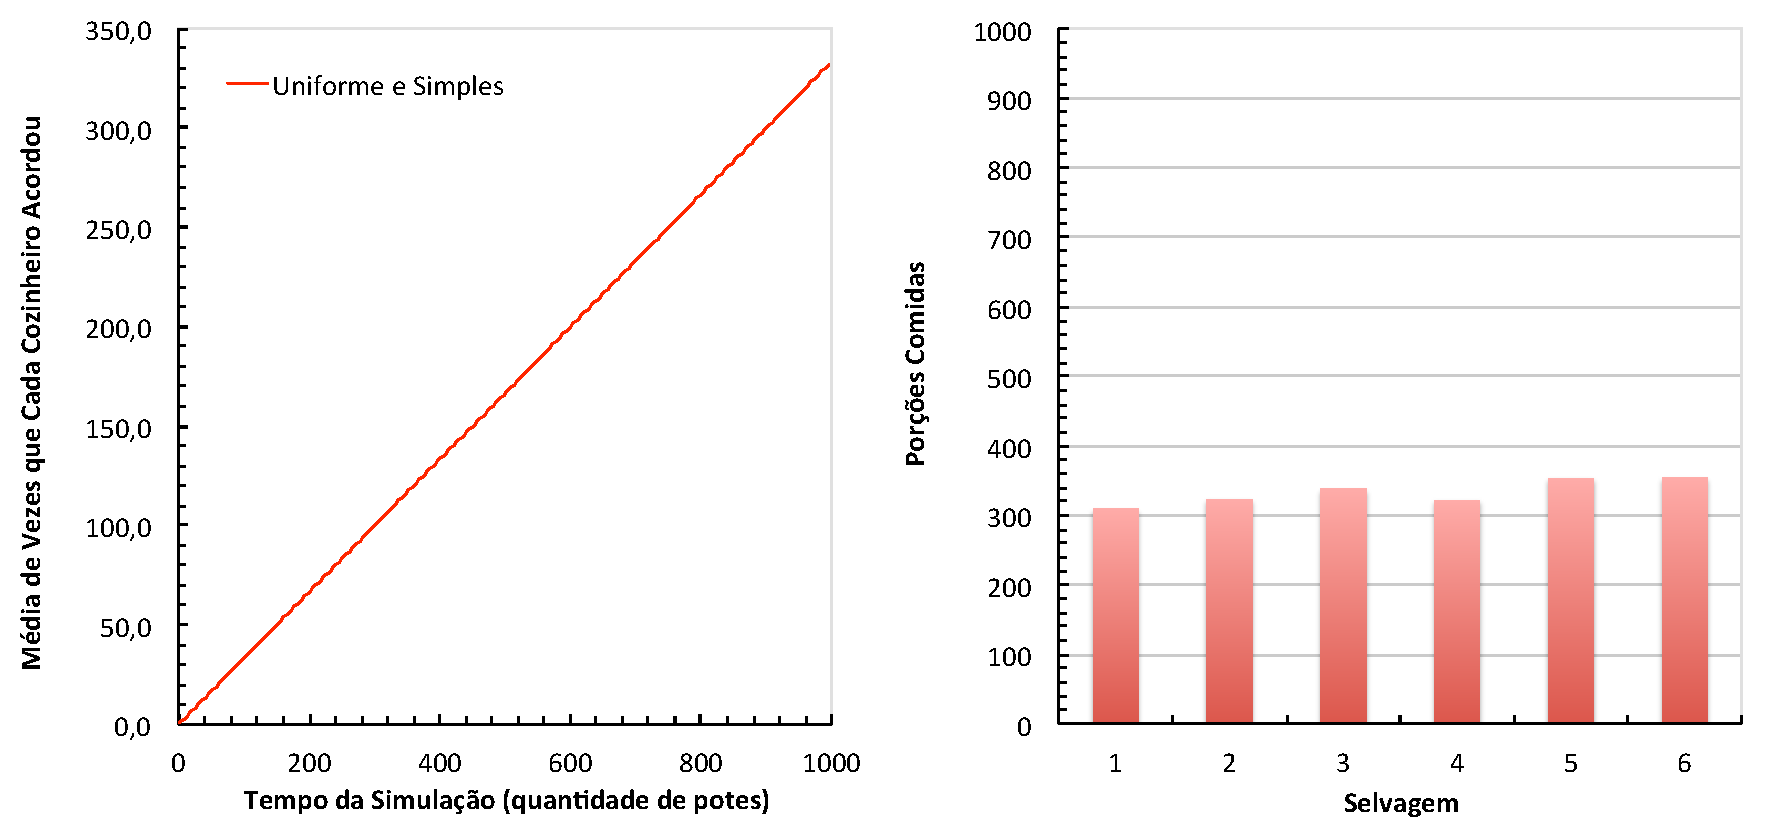
\includegraphics[scale=0.5]{uniforme_simples.pdf}
    \caption{}
  \end{center}
\end{figure}

\begin{figure}[htbp]
  \label{fig:ps}
  \begin{center}
    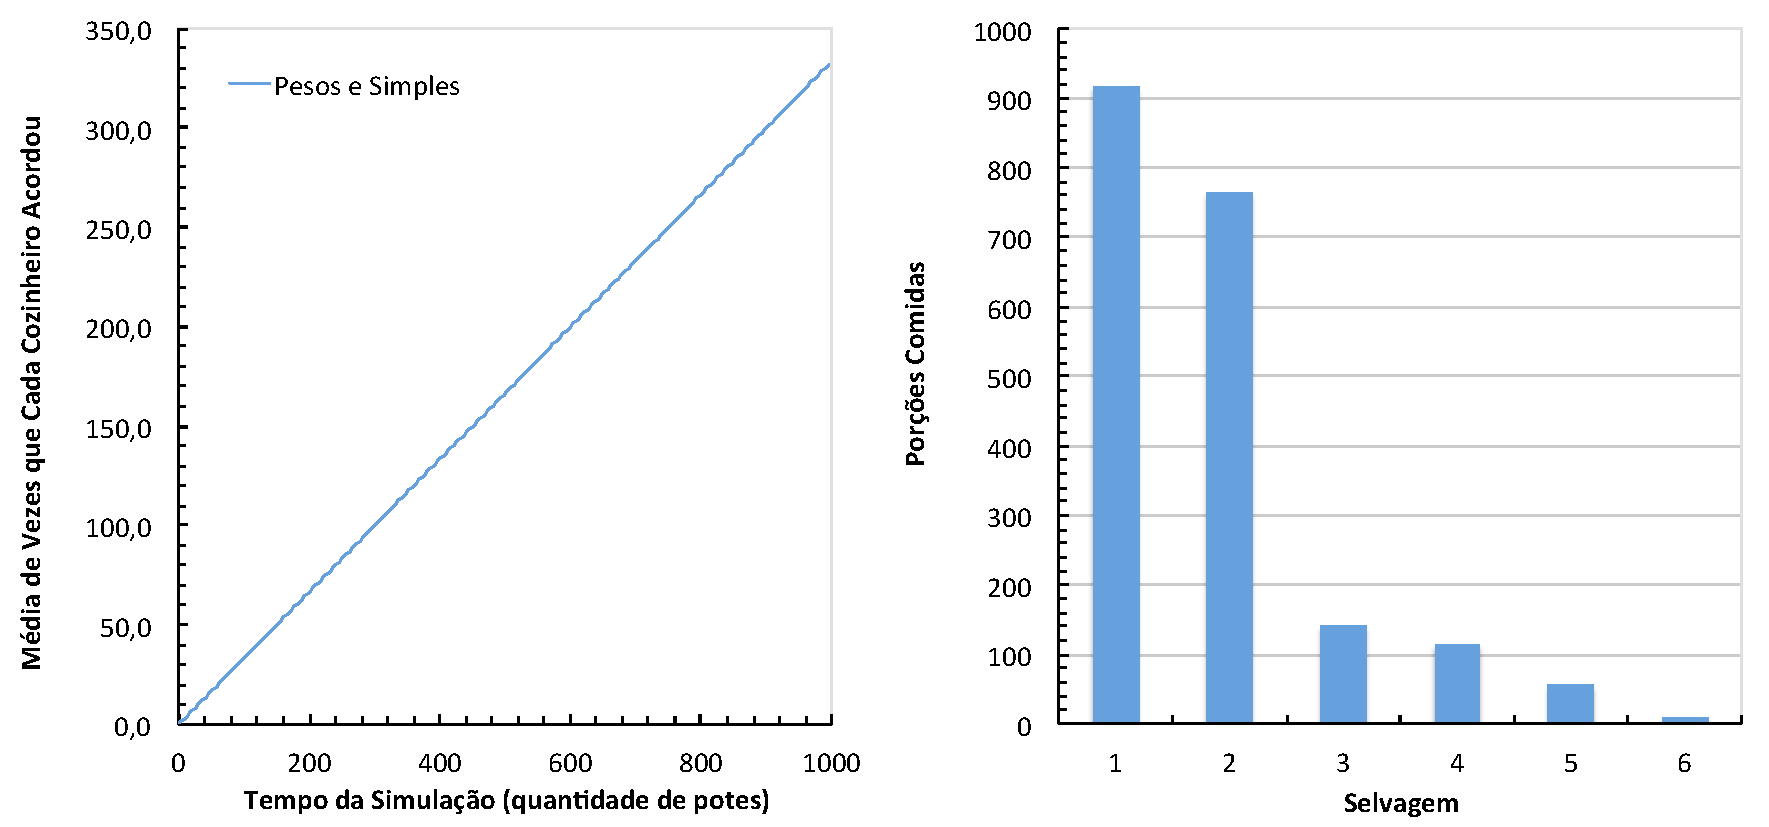
\includegraphics[scale=0.5]{pesos_simples.pdf}
    \caption{}
  \end{center}
\end{figure}

\begin{figure}[htbp]
  \label{fig:uc}
  \begin{center}
    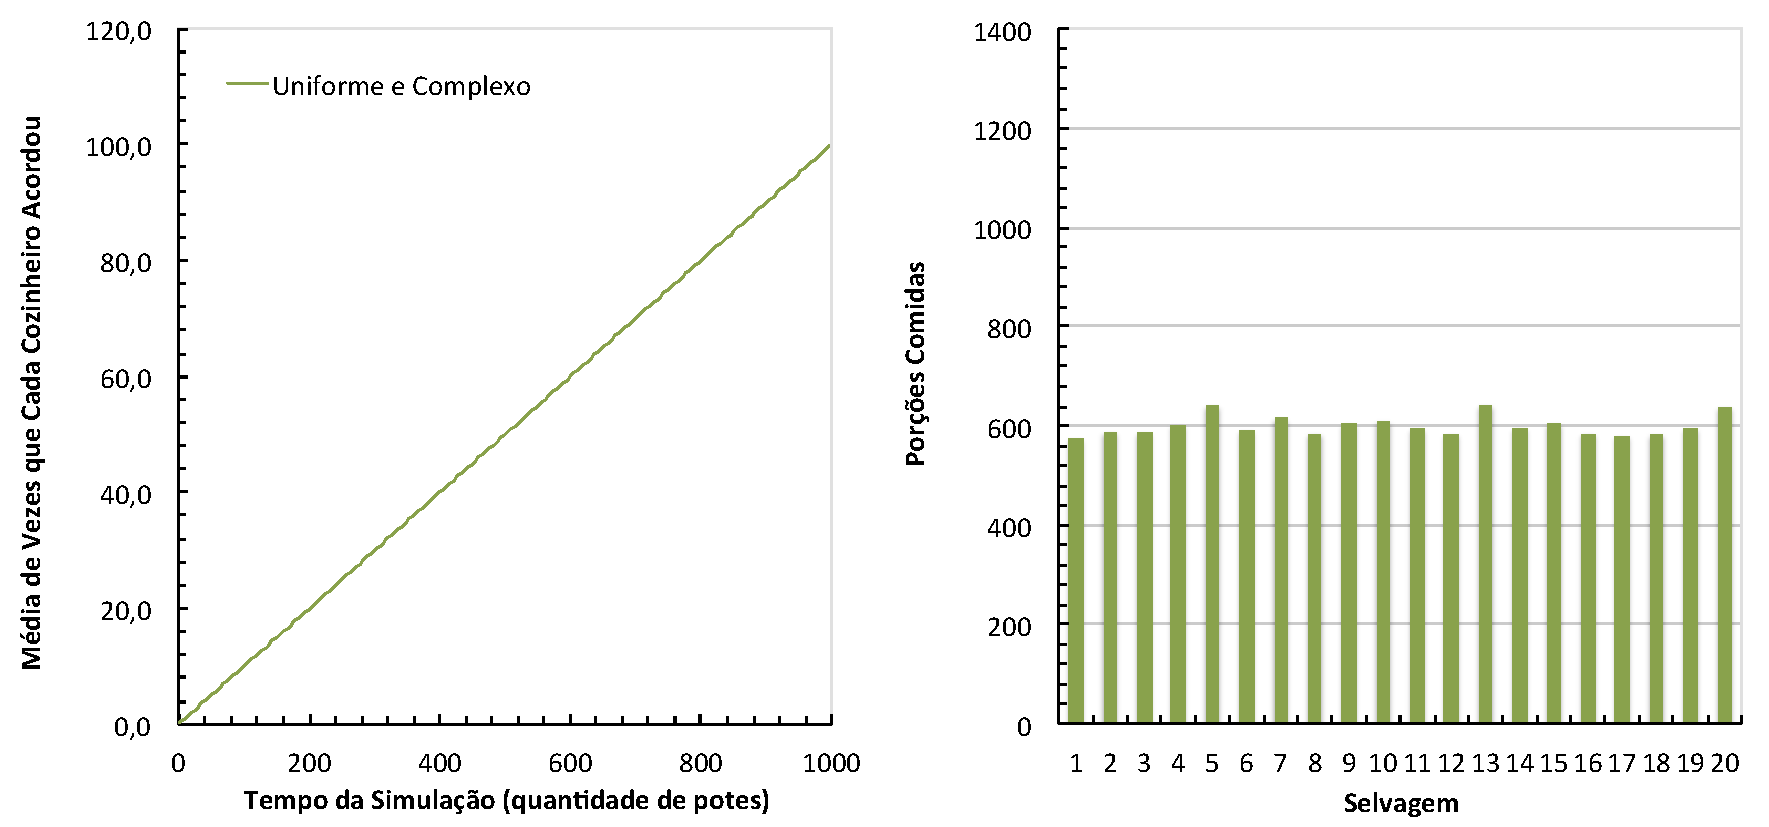
\includegraphics[scale=0.5]{uniforme_complexo.pdf}
    \caption{}
  \end{center}
\end{figure}

\begin{figure}[htbp]
  \label{fig:pc}
  \begin{center}
    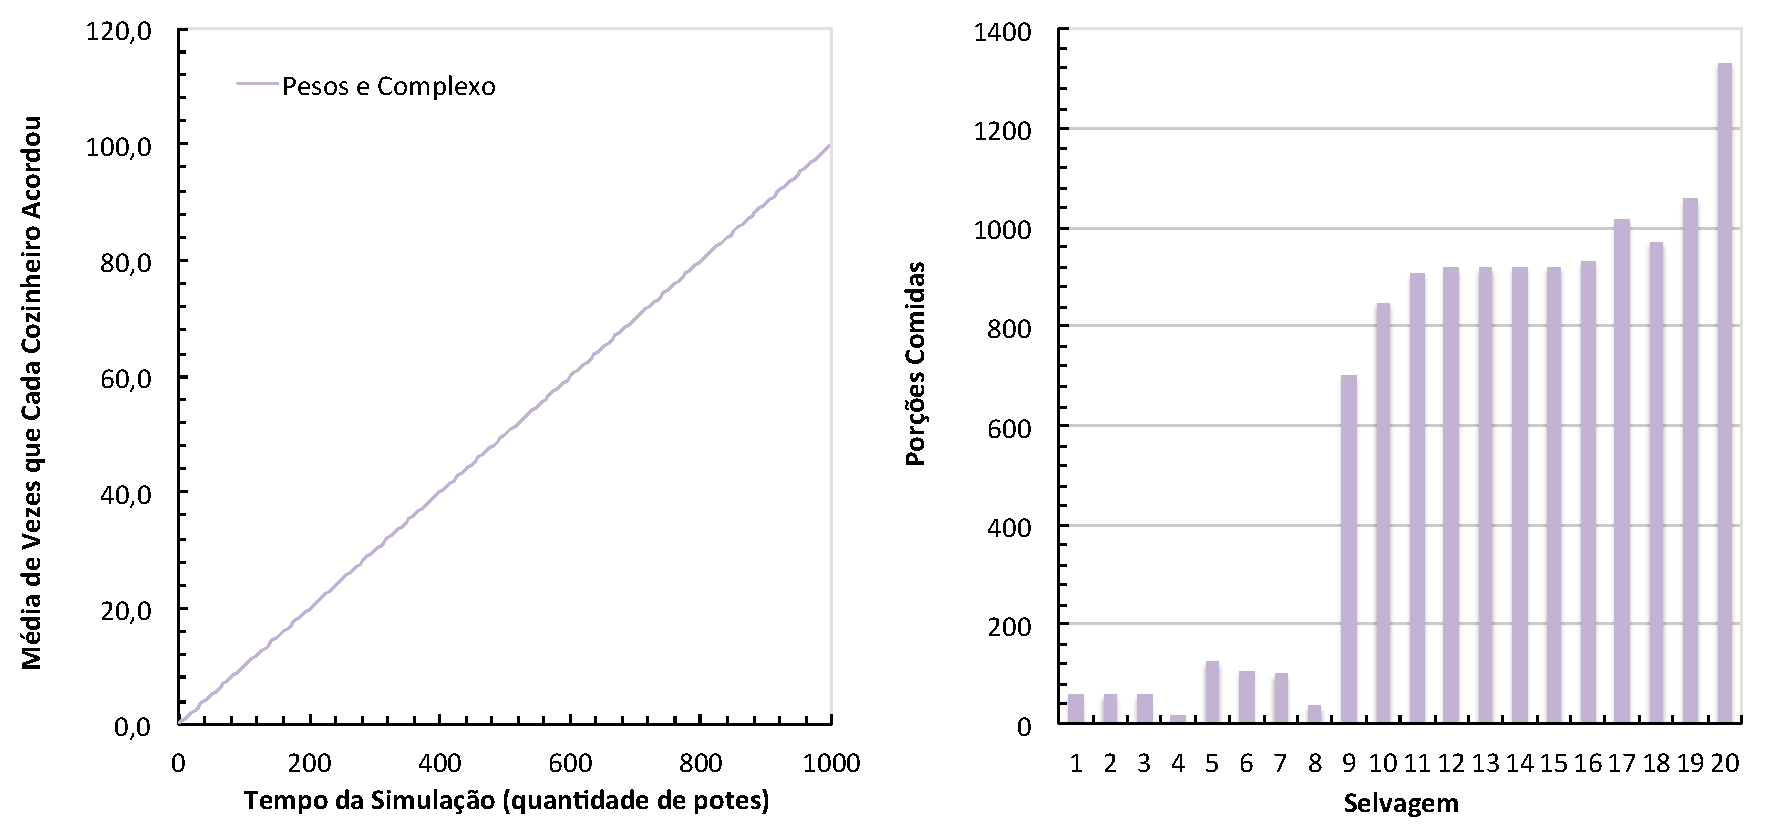
\includegraphics[scale=0.5]{pesos_complexo.pdf}
    \caption{}
  \end{center}
\end{figure}

%%%%%%%%%%%%%%%%%%%%%%%%%%%%%%%%%%%%%%%%%%%%%%%%%%%%%%%%%%%%%%%%%%%%%%%%%%%%%%%%%%%%%%%%%%%%%%%%%%%%

\section{Conclusões}
\label{sec:conc}

%%%%%%%%%%%%%%%%%%%%%%%%%%%%%%%%%%%%%%%%%%%%%%%%%%%%%%%%%%%%%%%%%%%%%%%%%%%%%%%%%%%%%%%%%%%%%%%%%%%%

%\begin{thebibliography}{99}
%  \bibitem{aima} S.~Russell, P.~Norvig. {\it Artificial Intelligence -- A Modern Approach}. Segunda
%  edição.
%\end{thebibliography}

\end{document}

